\documentclass{article}
% ~ ~ ~ ~ ~ ~ ~ ~ ~ ~ ~ ~ ~ ~ ~ ~ ~ ~ ~ ~ ~ ~ ~ ~ ~ ~ ~ ~ ~ ~ ~ ~ ~ ~ ~ ~ ~ ~ ~ ~ ~ ~ ~ ~ ~ ~ ~ ~

\usepackage[utf8]{inputenc}
\usepackage{amsmath}
\usepackage{amssymb} % for \mathbb
\usepackage{graphicx} % for figures
\usepackage{color}
\usepackage[usenames,dvipsnames]{xcolor}
\usepackage{hyperref} % for hyperlinks
\usepackage{float} % for figures
% ~ ~ ~ ~ ~ ~ ~ ~ ~ ~ ~ ~ ~ ~ ~ ~ ~ ~ ~ ~ ~ ~ ~ ~ ~ ~ ~ ~ ~ ~ ~ ~ ~ ~ ~ ~ ~ ~ ~ ~ ~ ~ ~ ~ ~ ~ ~ ~
% CUSTOM COLOUR
\definecolor{DGrey}{rgb}{0.1,0.1,0.1} % Dark Grey
% ~ ~ ~ ~ ~ ~ ~ ~ ~ ~ ~ ~ ~ ~ ~ ~ ~ ~ ~ ~ ~ ~ ~ ~ ~ ~ ~ ~ ~ ~ ~ ~ ~ ~ ~ ~ ~ ~ ~ ~ ~ ~ ~ ~ ~ ~ ~ ~
\title{ Introduction to Engineering Written Assignment Questions}
\date{January 2013}
\author{Greg Mayer and Daniel Connelly}
% ~ ~ ~ ~ ~ ~ ~ ~ ~ ~ ~ ~ ~ ~ ~ ~ ~ ~ ~ ~ ~ ~ ~ ~ ~ ~ ~ ~ ~ ~ ~ ~ ~ ~ ~ ~ ~ ~ ~ ~ ~ ~ ~ ~ ~ ~ ~ ~
% HEADER/FOOTER
\usepackage{fancyheadings}
\pagestyle{myheadings} % set headings to be user defined
\fancyhead{} % To create custom header, clear default layout
\renewcommand{\subsectionmark}[1]{\markright{{\color{DGrey}\thesubsection} \ {\color{DGrey}#1}}}
\fancyhead[LE,LO]{\subsectionmark} % To create custom header, clear default layout

% ~ ~ ~ ~ ~ ~ ~ ~ ~ ~ ~ ~ ~ ~ ~ ~ ~ ~ ~ ~ ~ ~ ~ ~ ~ ~ ~ ~ ~ ~ ~ ~ ~ ~ ~ ~ ~ ~ ~ ~ ~ ~ ~ ~ ~ ~ ~ ~
% ENUMERATION

\usepackage{enumitem}   % so that question numbers can be formatted 
\setenumerate[1]{label=\thesubsection.\arabic*.} % enumerate environment: add section numbers to items
% ~ ~ ~ ~ ~ ~ ~ ~ ~ ~ ~ ~ ~ ~ ~ ~ ~ ~ ~ ~ ~ ~ ~ ~ ~ ~ ~ ~ ~ ~ ~ ~ ~ ~ ~ ~ ~ ~ ~ ~ ~ ~ ~ ~ ~ ~ ~ ~
% MARGINS
\usepackage{anysize}
\marginsize{2.5cm}{2.5cm}{1cm}{1cm}
% ~ ~ ~ ~ ~ ~ ~ ~ ~ ~ ~ ~ ~ ~ ~ ~ ~ ~ ~ ~ ~ ~ ~ ~ ~ ~ ~ ~ ~ ~ ~ ~ ~ ~ ~ ~ ~ ~ ~ ~ ~ ~ ~ ~ ~ ~ ~ ~
% PAGE NUMBERING
\pagenumbering{arabic}
% ~ ~ ~ ~ ~ ~ ~ ~ ~ ~ ~ ~ ~ ~ ~ ~ ~ ~ ~ ~ ~ ~ ~ ~ ~ ~ ~ ~ ~ ~ ~ ~ ~ ~ ~ ~ ~ ~ ~ ~ ~ ~ ~ ~ ~ ~ ~ ~
% Custom Commands
\newcommand{\Emph}[1]{\textbf{#1}} % Emphasize
\newcommand{\R}{\mathbb{R}} 
\newcommand{\BM}{\begin{bmatrix}} % Begin Matrix
\newcommand{\EM}{\end{bmatrix}} % End Matrix
\newcommand{\BEN}{\begin{enumerate}[leftmargin=1.1cm]}% Begin ENumerate
\newcommand{\EEN}{\end{enumerate}} % End ENumerate
\newcommand{\MB}{\mathbf} % Math Bold

\newcommand{\px}{\frac{\partial}{\partial x}} % Partial wrt x
\newcommand{\py}{\frac{\partial}{\partial y}} % Partial wrt y

\newcommand{\pfx}{\frac{\partial f}{\partial x}} % Partial of f wrt x
\newcommand{\pfy}{\frac{\partial f}{\partial y}} % Partial of f wrt y
\newcommand{\pfxy}{\frac{\partial^2 f}{\partial y \partial x}} % Partial of f wrt y
\newcommand{\pfyx}{\frac{\partial^2 f}{\partial x \partial y}} % Partial of f wrt y

\newcommand{\ux}{\frac{\partial u}{\partial x }} % Partial of u wrt x
\newcommand{\uk}{\frac{\partial u}{\partial k }} % Partial of u wrt k
\newcommand{\ut}{\frac{\partial u}{\partial t}} % Partial of u wrt t
\newcommand{\utt}{\frac{\partial^2u}{\partial t^2}} % Partial of u wrt t
\newcommand{\us}{\frac{\partial u}{\partial s}} % Partial of u wrt t
\newcommand{\uss}{\frac{\partial^2 u}{\partial s^2}} % Partial of u wrt t
\newcommand{\kx}{\frac{\partial k}{\partial x }} % Partial of k wrt x
\newcommand{\kt}{\frac{\partial k}{\partial t }} % Partial of k wrt t

\newcommand{\pxu}{\frac{\partial x}{\partial u}} % x wrt u
\newcommand{\pxv}{\frac{\partial x}{\partial v}} % x wrt v
\newcommand{\pxw}{\frac{\partial x}{\partial w}} % x wrt v
\newcommand{\pxt}{\frac{\partial x}{\partial t}} % x wrt t
\newcommand{\pyu}{\frac{\partial y}{\partial u}} % y wrt u
\newcommand{\pyv}{\frac{\partial y}{\partial v}} % y wrt v
\newcommand{\pyw}{\frac{\partial y}{\partial w}} % y wrt v
\newcommand{\pyt}{\frac{\partial y}{\partial t}} % y wrt t
\newcommand{\pzu}{\frac{\partial z}{\partial u}} % z wrt u
\newcommand{\pzv}{\frac{\partial z}{\partial v}} % z wrt v
\newcommand{\pzw}{\frac{\partial z}{\partial w}} % z wrt v
\newcommand{\pzt}{\frac{\partial z}{\partial t}} % z wrt t


\newcommand{\VCT}{\textit{Vector Calculus} by Michael Corral} % Vector Calculus Textbook
\newcommand{\CAT}{\textit{College Algebra} by Carl Stitz and Jeff Zeager} % College Algebra Textbook
\newcommand{\From}{The following questions are related to } % Questions ....
% ~ ~ ~ ~ ~ ~ ~ ~ ~ ~ ~ ~ ~ ~ ~ ~ ~ ~ ~ ~ ~ ~ ~ ~ ~ ~ ~ ~ ~ ~ ~ ~ ~ ~ ~ ~ ~ ~ ~ ~ ~ ~ ~ ~ ~ ~ ~ ~
% ONLY USED FOR EDITING
\newcommand{\rednote}[1]{{\color{red}\textit{\textbf{#1}}}} % Shortcut for formatting notes for developers
\newcommand{\FromC}[1]{{\color{DGrey}\textit{#1}}} % Shortcut for coloring the "from" text
% ~ ~ ~ ~ ~ ~ ~ ~ ~ ~ ~ ~ ~ ~ ~ ~ ~ ~ ~ ~ ~ ~ ~ ~ ~ ~ ~ ~ ~ ~ ~ ~ ~ ~ ~ ~ ~ ~ ~ ~ ~ ~ ~ ~ ~ ~ ~ ~
% AUGMENTED MATRIX MACRO
% thanks to http://tex.stackexchange.com/questions/2233/whats-the-best-way-make-an-augmented-coefficient-matrix
\newenvironment{amatrix}[1]{%
  \left[\begin{array}{@{}*{#1}{c}|c@{}}
}{%
  \end{array}\right]
}
% ~ ~ ~ ~ ~ ~ ~ ~ ~ ~ ~ ~ ~ ~ ~ ~ ~ ~ ~ ~ ~ ~ ~ ~ ~ ~ ~ ~ ~ ~ ~ ~ ~ ~ ~ ~ ~ ~ ~ ~ ~ ~ ~ ~ ~ ~ ~ ~
% PAGE LAYOUT
\addtolength{\topmargin}{10pt}
\addtolength{\headsep}{10pt}
\addtolength{\textheight}{-20pt}



\title{Written Assignment Questions and Solutions}
\date{}
% ~~~~~~~~~~~~~~~~~~~~~~~~~~~~~~~~~~~~~~~~~~~~~~~~~~~~~~~~~~~~~~~~~~~~~~~~~~~~~~~~~
\begin{document}
\maketitle
\tableofcontents 

\part{Questions for Written Assignments}
\section{Multivariable Functions and Algebra}
\rednote{Unit 2 questions would go here}
\section{Partial Derivatives}
\rednote{Unit 3 questions would go here}
\section{Multiple Integrals}

% s~s~s~s~s~s~s~s~s~s~s~s~s~s~s~s~s~s~s~s~s~s~s~s~s~s~s~s~s~s~s~s~s~s~s~s~s~s~s~s~s~s~s~s
% s~s~s~s~s~s~s~s~s~s~s~s~s~s~s~s~s~s~s~s~s~s~s~s~s~s~s~s~s~s~s~s~s~s~s~s~s~s~s~s~s~s~s~s
\subsection*{Wolfram Alpha Syntax (optional)}
You may want to use Wolfram Alpha (wolframalpha.com) to check your answers. If you're not sure what syntax to use to compute double integrals with Wolfram Alpha, let's suppose that we want to determine the value of
\begin{align*} 
   \mathop{\int_{-2}^{-1} \!  \int_0^{x-1}}( x^{2C} +y)  dy  dx
\end{align*}
where $C$ is a constant. The syntax we could use to compute this particular integral is
\begin{quote}
  \begin{verbatim}
    integrate x^{2C}+y dydx, x from -2 to -1 and y from 0 to (x-1)
  \end{verbatim}
\end{quote}
% s~s~s~s~s~s~s~s~s~s~s~s~s~s~s~s~s~s~s~s~s~s~s~s~s~s~s~s~s~s~s~s~s~s~s~s~s~s~s~s~s~s~s~s
% s~s~s~s~s~s~s~s~s~s~s~s~s~s~s~s~s~s~s~s~s~s~s~s~s~s~s~s~s~s~s~s~s~s~s~s~s~s~s~s~s~s~s~s
\subsection{Double Integrals}
\purple{\From Section 3.1 of \VCT.}

\BEN
% ~~~~~~~~~~~~~~~~~~~~~~~~~~~~~~~~~~~~~~~~~~~~~~~~~~~~~~~~~~~~~~~~~~~~~~~~~~~~~~~~~
\item % VOLUME OF SIMPLE SOLID 
Consider the solid that lies under the plane $z = -x-2y+2$ and above the rectangle \\$\{(x,y) \ | \ -2\le x\le 0, 0\le y \le1 \}$.
\BEN
\item Sketch the solid in $\R^3$. 
\item Find the volume of the solid.
\EEN
% ~~~~~~~~~~~~~~~~~~~~~~~~~~~~~~~~~~~~~~~~~~~~~~~~~~~~~~~~~~~~~~~~~~~~~~~~~~~~~~~~~
\item % FLUID MECHANICS
\textbf{Application to Fluid Mechanics} \\
In a two-dimensional, steady-state, incompressible fluid flow, the velocity \textbf{v} of the flow can be expressed as $\MB{v} = u(x,y)\MB{i} + v(x,y)\MB{j}$. The functions $u(x,y)$ and $v(x,y)$ must satisfy 
\begin{align*}
  \nabla\cdot\MB{v} = 0.
\end{align*}
\BEN
\item If $u(x,y) = x^2 + y^2$, find the most general form of $v(x,y)$. 
\item If $v(x,y) = \cos(x)$, find the most general form of $u(x,y)$.
\EEN
\textit{Hint: you are asked to find the most \Emph{general} form of functions u and v}.

\EEN % END OF QUESTIONS
% s~s~s~s~s~s~s~s~s~s~s~s~s~s~s~s~s~s~s~s~s~s~s~s~s~s~s~s~s~s~s~s~s~s~s~s~s~s~s~s~s~s~s~s
\subsection{Double Integrals Over a General Region}
\purple{\From Section 3.2 of \VCT.}

\BEN
% ~~~~~~~~~~~~~~~~~~~~~~~~~~~~~~~~~~~~~~~~~~~~~~~~~~~~~~~~~~~~~~~~~~~~~~~~~~~~~~~~~
\item % TETRAHEDRON
\Emph{Volume of a Tetrahedron} \\
A \Emph{tetrahedron} is a three dimensional object with four, triangular, flat sides. Because each of its four sides are flat, a tetrahedron can be defined as the region enclosed by four planes. Below is a sketch of two tetrahedrons. Note that each tetrahedron has four vertices, six edges, and that the lengths of its edges do not have to be equal.
\begin{figure}[h]
  \vspace{-1pt}
  \begin{center}
    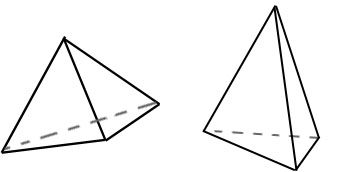
\includegraphics[width=0.35\textwidth]{ImgTetrahedrons.jpg}
  \end{center}
\end{figure}\\
Consider the tetrahedron that is bounded by the three coordinate planes in $\R^3$, and by the plane $z = 1 - x - \frac{y}{2}$.
\BEN
\item Sketch the tetrahedron in $\R^3$ and label the points that represent its four vertices. 
\item Set up, but do not evaluate, a double integral that represents the volume of the tetrahedron. Integrate with respect to $x$ first. 
\item Set up, but do not evaluate, a double integral that represents the volume of the tetrahedron. Integrate with respect to $y$ first. 
\EEN
Note that
\begin{itemize}
\item Examples 3.4 and 3.5 from \VCT \ are similar to this problem. 
\item We could also calculate the volume of the solid by using a \Emph{triple} integral. 
\item Although not required, the double integrals are straightforward to compute. You may want to check your answers by evaluating the integrals and seeing if you would get the same result in parts (b) and (c). 
\end{itemize}
% ~~~~~~~~~~~~~~~~~~~~~~~~~~~~~~~~~~~~~~~~~~~~~~~~~~~~~~~~~~~~~~~~~~~~~~~~~~~~~~~~~
\item  % DESCRIBE WHY A PARTICULAR DOUBLE INTEGRAL GIVES AREA
\Emph{Area of a General Region}
\BEN
\item Question 11 from Section 3.2 of \VCT. \textit{Hint: Figure 3.2.5 is also helpful.}
\item Use the result from part (a) to compute the area of the region bounded by the curves $y = x^2$ and $x=y^2$.
\EEN

% ~~~~~~~~~~~~~~~~~~~~~~~~~~~~~~~~~~~~~~~~~~~~~~~~~~~~~~~~~~~~~~~~~~~~~~~~~~~~~~~~~
\item % UPPER AND LOWER BOUNDS ARE FUNCTIONS
Find the volume of the solid enclosed by $z = x^2 + y^2$, $y = x^2$ and $x=y^2$.
% ~~~~~~~~~~~~~~~~~~~~~~~~~~~~~~~~~~~~~~~~~~~~~~~~~~~~~~~~~~~~~~~~~~~~~~~~~~~~~~~~~
\item % CHANGING ORDER OF INTEGRATION
Consider the integral
\begin{align*}
  \iint\limits_R x\sin(y) dA
\end{align*}
 where $R$ is the region bounded by $y=0$, $y=x^2$, and $x=2$.
\BEN
\item Evaluate the double integral by first integrating with respect to $x$. 
\item Evaluate the double integral by first integrating with respect to $y$. 
\EEN
Note that your answers for both parts should be the same, and that you may need to use various techniques of integration to complete this problem, including integration by parts and a variable substitution. 
% ~~~~~~~~~~~~~~~~~~~~~~~~~~~~~~~~~~~~~~~~~~~~~~~~~~~~~~~~~~~~~~~~~~~~~~~~~~~~~~~~~
\item % CHANGING ORDER OF INTEGRATION, GENERAL F(X,Y)
Consider the double integral
\begin{align*}
  \mathop{\int_{0}^{1+e} \! \int_0^{\ln(x-1)}} f(x,y) dydx .
\end{align*}
Sketch the region in $\R^2$ over which $f(x,y)$ is integrated, and change the order of integration.  
% ~~~~~~~~~~~~~~~~~~~~~~~~~~~~~~~~~~~~~~~~~~~~~~~~~~~~~~~~~~~~~~~~~~~~~~~~~~~~~~~~~
\item % BOUNDING AN INTEGRAL 
Consider the double integral
\begin{align*}
  \iint\limits_D f(x,y) dA,
\end{align*}
where $D$ is the square $0\le x \le 1$, $0\le y \le 1$, and $f(x,y) = \sin(x+y)$. Show that 
\begin{align*}
  0 \le \iint\limits_D f(x,y) dA \le 1.
\end{align*}
% ~~~~~~~~~~~~~~~~~~~~~~~~~~~~~~~~~~~~~~~~~~~~~~~~~~~~~~~~~~~~~~~~~~~~~~~~~~~~~~~~~
\item % SYMMETRY
\textbf{Simplifying Double Integrals Using Symmetry} \\
Certain integrals can be simplified when the integrand is either even or odd. You may know that, for functions of one variable, that
\begin{align*}
  \text{if }f(x)\text{ is odd, then } & \int_{-a}^{a} f(x) dx = 0 . \\
  \text{if }f(x)\text{ is even, then } & \int_{-a}^{a} f(x) dx = 2 \int_0^a f(x) dx.
\end{align*}
There are similar results for integrals of two variables, but in order to introduce them, we first need to extend our concepts of even and odd functions to functions of two variables, and we need to describe regions that are symmetric about the $x$-axis and about the $y$-axis. 

If $R$ is a region that is \Emph{symmetric about the $y$-axis}, and $(x_0,y_0)$ is a point inside $R$, then the point $(-x_0,y_0)$ is also inside $R$. Similarily, if $S$ is a region that is \Emph{symmetric about the $x$-axis}, and $(x_1,y_1)$ is a point inside $S$, then the point $(x_1,-y_1)$ is also inside $S$. Above are examples of regions that have these symmetries.\\

\begin{figure}[h]
  \vspace{-1pt}
  \begin{center}
    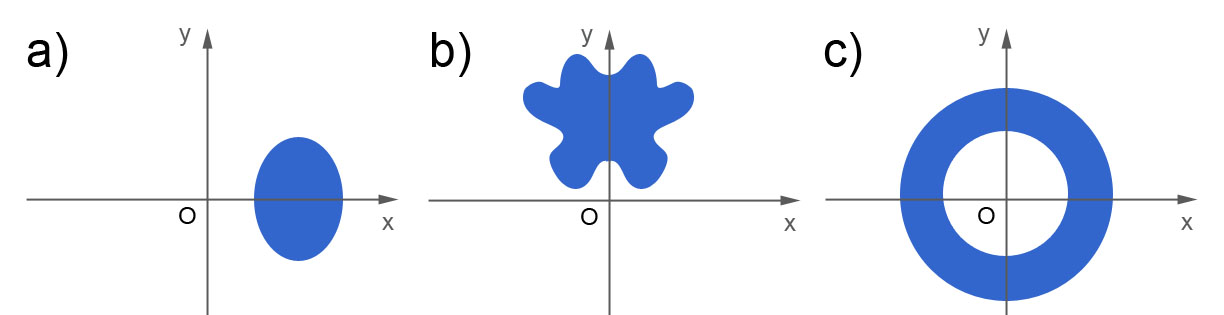
\includegraphics[width=0.95\textwidth]{ImgRegions.jpg}
  \end{center}
 \begin{quote} \caption{\small{a) the blue region is symmetric about the $x$-axis, b) the blue region is symmetric about the $y$-axis, and c) the blue region is symmetric about the $x$-axis and the $y$-axis.}}\end{quote}
\end{figure}

Moreover, if $g(x,y)$ is odd in $x$, then 
\begin{align*}
  g(-x,y) = - g(x,y).
\end{align*}
But if $g(x,y)$ were even in $x$, then 
\begin{align*}
  g(-x,y) =  g(x,y).
\end{align*}
Combining these concepts yields helpful results for computing double integrals. For example, if $R$ is symmetric about the $y$-axis, and if $g(x,y)$ is odd in $x$, then
\begin{align*}
  \iint\limits_R g(x,y) dxdy = 0.
\end{align*}
Similar results can be stated if $g$ were even in $x$ or in $y$, and if $R$ has symmetry about the $x$-axis. 
\BEN
\item Provide an example of a non-zero function of two variables, $h(x,y)$, that is odd in $x$. Verify that your function is odd in $x$.
\item Provide an example of a region, $D$, that is symmetric about the $y$-axis, but is not symmetric about the $x$-axis. 
\item Show that, for your $h(x,y)$ and region $D$, that 
\begin{align*}
  \iint\limits_D g(x,y) dxdy = 0.
\end{align*}
\EEN

\EEN % END OF QUESTIONS
% s~s~s~s~s~s~s~s~s~s~s~s~s~s~s~s~s~s~s~s~s~s~s~s~s~s~s~s~s~s~s~s~s~s~s~s~s~s~s~s~s~s~s~s
% s~s~s~s~s~s~s~s~s~s~s~s~s~s~s~s~s~s~s~s~s~s~s~s~s~s~s~s~s~s~s~s~s~s~s~s~s~s~s~s~s~s~s~s
\subsection{Triple Integrals}
\purple{\From Section 3.3 of \VCT.}
  
\BEN
% ~~~~~~~~~~~~~~~~~~~~~~~~~~~~~~~~~~~~~~~~~~~~~~~~~~~~~~~~~~~~~~~~~~~~~~~~~~~~~~~~~
\item % TETRAHEDRON
\Emph{Volume of a Tetrahedron} \\
The textbook points out that the triple integral 
\begin{align*}
  \iiint\limits_S f(x,y,z) dV
\end{align*}
for the special special case when $f(x,y,z) = 1$ for all points in $S$, gives the volume of $S$
\begin{align*}
  V(S) &= \iiint\limits_S dV.
\end{align*}
Consider again the tetrahedron that is bounded by the three coordinate planes in $\R^3$, and by the plane $z = 1 - x - \frac{y}{2}$. We derived an expression for the volume of this tetrahedron in a previous question using a double integral. Now set-up and find the volume of the tetrahedron using a triple integral.
% ~~~~~~~~~~~~~~~~~~~~~~~~~~~~~~~~~~~~~~~~~~~~~~~~~~~~~~~~~~~~~~~~~~~~~~~~~~~~~~~~~
\item % VOLUME OF AN ELLIPSOID
\textbf{Volume of an Ellipsoid}\\
Solve Question 10 from Section 3.5 of \VCT.
% ~~~~~~~~~~~~~~~~~~~~~~~~~~~~~~~~~~~~~~~~~~~~~~~~~~~~~~~~~~~~~~~~~~~~~~~~~~~~~~~~~
\item % VOLUME OF SOLID
\textbf{Volume of a Solid}\\
Find the volume of the solid enclosed by the planes
\begin{align*}
  z & = x+y\\
  y &= x \\
  x &= 0 \\
  z &= 0 \\
  y &= 2
\end{align*}
\textit{Hint: it may help to start by plotting the planes in Google or in Wolfram Alpha.}
\EEN
% s~s~s~s~s~s~s~s~s~s~s~s~s~s~s~s~s~s~s~s~s~s~s~s~s~s~s~s~s~s~s~s~s~s~s~s~s~s~s~s~s~s~s~s
% s~s~s~s~s~s~s~s~s~s~s~s~s~s~s~s~s~s~s~s~s~s~s~s~s~s~s~s~s~s~s~s~s~s~s~s~s~s~s~s~s~s~s~s
\subsection{Change of Variables in Multiple Integrals}
\purple{\From Section 3.5 of \VCT.}
\BEN
% ~~~~~~~~~~~~~~~~~~~~~~~~~~~~~~~~~~~~~~~~~~~~~~~~~~~~~~~~~~~~~~~~~~~~~~~~~~~~~~~~~
\item % GENERAL TRANSFORMATION
\Emph{Linear Transformations} \\
Under the linear transformation 
\begin{align*}
  x = c_1u + c_2v , \quad y =d_1u + d_2v, \quad d_1c_2 - d_2c_1 \ne 0,
\end{align*}
straight lines in the $uv$-plane are mapped to straight lines in the $xy$-plane. 
\BEN
\item $v=v_0$ is a horizontal line in the $uv$-plane. Determine the equation of this line in the $xy$-plane. 
\item $x=x_0$ is a vertical line in the $xy$-plane. Determine the equation of this line in the $uv$-plane.
\EEN
% ~~~~~~~~~~~~~~~~~~~~~~~~~~~~~~~~~~~~~~~~~~~~~~~~~~~~~~~~~~~~~~~~~~~~~~~~~~~~~~~~~
\item % STRAIGHTFORWARD CHANGE OF VARIABLES
Use an appropriate transformation to evaluate the integral
\begin{align*}
  \iint\limits_R \big(x^2 - y^2\big) dxdy,
\end{align*}
where $R$ is the parallelogram bounded by 
\begin{align*}
  x+y = 0, \quad x+y = 1, \quad x-y=0, \quad x-y=1.
\end{align*}

% ~~~~~~~~~~~~~~~~~~~~~~~~~~~~~~~~~~~~~~~~~~~~~~~~~~~~~~~~~~~~~~~~~~~~~~~~~~~~~~~~~
\item % CHANGE OF VARIABLES TWICE
\Emph{Simplifying Double Integrals} \\
When working with double integrals over a rectangular region $R=\{(x,y) | a \le x \le b, c\le y \le d\}$, we can use the simplification
\begin{align*}
   \iint\limits_{R} g(x) h(y) dA 
  & = \int_a^b g(x) dx \int_c^d h(y) dy  
\end{align*}
Use this property and the transformation $x = 3u, y = 2v$ to evaluate the double integral
\begin{align*}
  \iint\limits_E x^2 \ dxdy,
\end{align*}
where $E$ is region bounded by the ellipse $4x^2 + 9y^2 = 36$. 
% ~~~~~~~~~~~~~~~~~~~~~~~~~~~~~~~~~~~~~~~~~~~~~~~~~~~~~~~~~~~~~~~~~~~~~~~~~~~~~~~~~
\item % SIMPLE CYLINDRICAL WITH CONE
Evaluate the integral
\begin{align*}
  \iiint\limits_S y^2dV,
\end{align*}
where $S$ is the solid that lies inside the cylinder $x^2+y^2 = 1$, above the plane $z=0$ and below the cone $z^2 = 9x^2 + 9y^2$. 
% ~~~~~~~~~~~~~~~~~~~~~~~~~~~~~~~~~~~~~~~~~~~~~~~~~~~~~~~~~~~~~~~~~~~~~~~~~~~~~~~~~
\item % TRIPLE INTEGRAL IN CYLINDRICAL COORDINATES
\Emph{Triple Integral In Cylindrical Coordinates} \\
Evaluate the integral
\begin{align*}
  \iiint\limits_V dV,
\end{align*}
using cylindrical coordinates, where $V$ is the region bounded by
\begin{align*}
  0 \le\ &x \le 2 \\
  0 \le\ &y \le \sqrt{4 - x^2}\\
  0 \le\ &z \le \sqrt{4 - (x^2+ y^2)}
\end{align*} 
% ~~~~~~~~~~~~~~~~~~~~~~~~~~~~~~~~~~~~~~~~~~~~~~~~~~~~~~~~~~~~~~~~~~~~~~~~~~~~~~~~~
\item % TRIPLE INTEGRAL IN SPHERICAL COORDINATES
\Emph{Triple Integral In Spherical Coordinates} \\
The integral
\begin{align*}
  \mathop{\int_0^{\pi/4} \!\! \int_{0}^{\pi/2} \!\! \int_0^1 } ( \rho^2 \sin\phi ) \ d\rho\  d\phi\  d\theta
\end{align*}
represents the volume of a solid. Describe the shape of the solid, and find its volume. \\\rednote{Textbook doesn't do a great job of integrals in cylindrical and spherical}

% ~~~~~~~~~~~~~~~~~~~~~~~~~~~~~~~~~~~~~~~~~~~~~~~~~~~~~~~~~~~~~~~~~~~~~~~~~~~~~~~~~
\item % EVEN AND ODD
\rednote{I'll push this question to a midterm or final exam}\\
Determine the value of
\begin{align*}
  \mathop{\int_0^{\pi} \!\! \int_{-1}^1} x^4e^{x^2 + y^2}\sin(y) dydx.
\end{align*}
\textit{Hint: integration by parts is not necessary.}
% ~~~~~~~~~~~~~~~~~~~~~~~~~~~~~~~~~~~~~~~~~~~~~~~~~~~~~~~~~~~~~~~~~~~~~~~~~~~~~~~~~


% ~~~~~~~~~~~~~~~~~~~~~~~~~~~~~~~~~~~~~~~~~~~~~~~~~~~~~~~~~~~~~~~~~~~~~~~~~~~~~~~~~

\EEN % END OF QUESTIONS

\section{Line and Surface Integrals}
\rednote{Unit 5 questions would go here}
%%%%%%%%%%%%%%%%%%%%%%%%%%%%%%%%%%%%%%%%%%%%%%%%%%%%%%%%%%%%%%%%
%%%%%%%%%%%%%%%%%%%%%%%%%%%%%%%%%%%%%%%%%%%%%%%%%%%%%%%%%%%%%%%%
%%%%%%%%%%%%%%%%%%%%%%%%%%%%%%%%%%%%%%%%%%%%%%%%%%%%%%%%%%%%%%%%
%%%%%%%%%%%%%%%%%%%%%%%%%%%%%%%%%%%%%%%%%%%%%%%%%%%%%%%%%%%%%%%%
% SOLUTIONS
\part{Solutions to Written Assignment Questions}
\setcounter{section}{0}
\section{Multivariable Functions and Algebra}
\rednote{Unit 2 sol'ns would go here}
\section{Partial Derivatives}
\rednote{Unit 3 sol'ns would go here}
\section{Multiple Integrals}
\newpage

\subsection{Double Integrals}

\BEN 
% ~~~~~~~~~~~~~~~~~~~~~~~~~~~~~~~~~~~~~~~~~~~~~~~~~~~~~~~~~~~~~~~~~~~~~~~~~~~~~~~~~
\item % VOLUME OF SIMPLE SOLID 
\BEN
\item A sketch of the volume is below. 
\begin{figure}[h]
  \vspace{-1pt}
  \begin{center}
    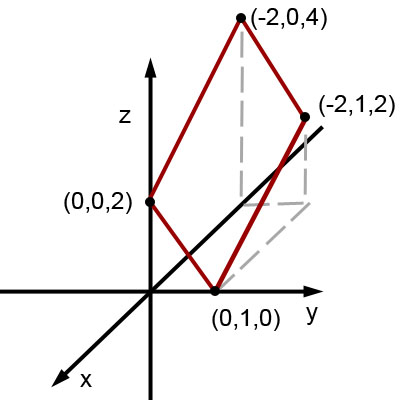
\includegraphics[width=0.35\textwidth]{ImgSolid.jpg}
  \end{center}
\end{figure}
\item We must integrate:
\begin{align*}
  \mathop{\int_{-2}^0 \! \int_0^1} (-x-2y+2 ) dydx 
  &= \int_{-2}^0 \big( -2xy -y^2 + 2y \big) \big|_0^1 dx \\
  &= \int_{-2}^0 \Big( -2x + 1  \Big) dx \\
  &= \Big(-x^2 + x \Big) \Big|_{-2}^0  \\  
  &= 0- \big(- (-2)^2 + (-2)\big)\\
  &= 0- \big(- 4 -2\big)\\
  &= 6
\end{align*}
\EEN
% ~~~~~~~~~~~~~~~~~~~~~~~~~~~~~~~~~~~~~~~~~~~~~~~~~~~~~~~~~~~~~~~~~~~~~~~~~~~~~~~~~
\item % FLUID MECHANICS
\BEN
\item Substituting the expression for $u$ into the divergence equation yields
\begin{align*}
  0&= \nabla \cdot \MB{v} \\
  &= \px \big(u(x,y)\big) + \py \big(v(x,y)\big) \\
  &= \px (x^2 + y^2) + \frac{\partial v}{\partial y}\\
  &= 2x + \frac{\partial v}{\partial y} \\
   \frac{\partial v}{\partial y} &= -2x 
\end{align*}
Therefore, $v(x,y)$ is a function whose partial derivative with respect to $y$ is $-2x$. The \Emph{most general} form for $v(x,y)$ is obtained by integrating with respect to $y$:
\begin{align*}
 v(x,y) &= -2xy + f(x)
\end{align*}
where $f(x)$ is an unknown function of one variable, $x$. 
\item Using the same approach as we used for (a) yields
\begin{align*}
  0&= \nabla \cdot \MB{v} \\
  &= \px \big(u(x,y)\big) + \py \big(v(x,y)\big) \\
  &=  \frac{\partial u}{\partial x}+ 0\\
   \frac{\partial u}{\partial x} &= 0
\end{align*}
Therefore, $u(x,y)$ is a function whose partial derivative with respect to $x$ is $0$. The \Emph{most general} form for $u(x,y)$ is obtained by integrating with respect to $x$:
\begin{align*}
 u(x,y) &= g(y)
\end{align*}
where $g(y)$ is an unknown function of one variable, $y$. 
\EEN

\EEN % END OF QUESTIONS
% s~s~s~s~s~s~s~s~s~s~s~s~s~s~s~s~s~s~s~s~s~s~s~s~s~s~s~s~s~s~s~s~s~s~s~s~s~s~s~s~s~s~s~s
\subsection{Double Integrals Over a General Region}
\BEN
% ~~~~~~~~~~~~~~~~~~~~~~~~~~~~~~~~~~~~~~~~~~~~~~~~~~~~~~~~~~~~~~~~~~~~~~~~~~~~~~~~~
\item % TETRAHEDRON
\BEN
\item A sketch of the tetrahedron is below. 
\begin{figure}[h]
  \vspace{-1pt}
  \begin{center}
    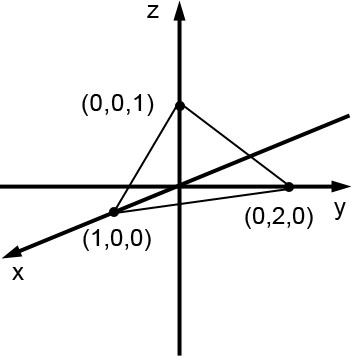
\includegraphics[width=0.35\textwidth]{ImgTetExample.jpg}
  \end{center}
\end{figure}
% ~  ~  ~  ~  ~  ~  ~  ~  ~  ~  ~  ~  ~  ~  ~  ~  ~  ~  ~  ~  ~  ~  ~  ~  
\item The tetrahedron has one side in the $xy$-plane. This side is bounded by the line that is the intersection between the $xy$-plane and the plane $z = 1 - x - y/2$. We can find this intersection by setting $z=0$,
\begin{align*}
  0 &= 1 - x - \frac{y}{2} \\
  x &= 1 - \frac{y}{2}.
\end{align*}
Therefore, the volume is the region under the plane $z = 1 - x - y/2$ and over  
\begin{align*}
  R = \{ (x,y) \ | \ 0 \le x \le 1- y/2, \ 0 \le y \le 2 \}.
\end{align*}
The double integral is 
\begin{align*}
  \mathop{\int_{0}^{2} \! \int_0^{1-y/2} } (1 - x - \frac{y}{2}) dxdy
\end{align*} 
% ~  ~  ~  ~  ~  ~  ~  ~  ~  ~  ~  ~  ~  ~  ~  ~  ~  ~  ~  ~  ~  ~  ~  ~  
\item The volume is the region under the plane $z = 1 - x - y/2$ and over  
\begin{align*}
  R = \{ (x,y) \ | \ 0 \le x \le 1, \ 0 \le y \le 2 - 2x \}.
\end{align*}
The double integral is 
\begin{align*}
  \mathop{\int_{0}^{1} \! \int_0^{2-2x} } (1 - x - \frac{y}{2}) dydx
\end{align*} 
\EEN
% ~~~~~~~~~~~~~~~~~~~~~~~~~~~~~~~~~~~~~~~~~~~~~~~~~~~~~~~~~~~~~~~~~~~~~~~~~~~~~~~~~
\item % DOUBLE INTEGRAL IS AREA IF F=1
\BEN
\item
Suppose that we subdivide region $R$ into a rectangular grid of sub-rectangles (as in Figure 3.2.5), so that we only consider the sub-rectangles that are completely enclosed in $R$. Then, the area of region $R$ is approximated by the double sum
\begin{align*}
  \sum_j\sum_i\Delta x_i \Delta y_j
\end{align*}
But if $f=1$ for all $x_i$ and $y_j$, this is equal to:
\begin{align}\label{abefaberabreabr}
  \sum_j\sum_i f(x_i,y_j) \Delta x_i \Delta y_j
\end{align}
where $x_i$ and $y_j$ is a point inside sub-rectangle $[x_i,x_{i+1}]\times[y_j,y_{j+1}]$. 
If we take smaller and smaller rectangles, so that the length of the longest diagonal of the sub-rectangles goes to zero, the sub-rectangles begin to fill more and more of the region $R$, and so the above sums approach the  \Emph{area} of region $R$. Since we have defined
\begin{align*}
  \mathop{\int \!\!\! \int} f(x,y) dA
\end{align*}
as the limit of Equation (\ref{abefaberabreabr}) as the longest diagonal goes to zero, and $f(x,y)=1$, the double integral 
\begin{align*}
  \mathop{\int \!\!\! \int} 1 dA
\end{align*}
is the area of region $R$. 
\item The region may be defined as
\begin{align*}
  R = \{ (x,y) \ | \ 0 \le x \le 1, \ x^2 \le y \le \sqrt{x} \}.
\end{align*}
The area of $R$ is 
\begin{align*}
  \mathop{\int_0^1 \!\!\! \int_{x^2}^{\sqrt{x}}} dydx 
  &= \int_0^1 \Big(\sqrt{x} - x^2 \Big) dx \\
  &= \Big(\frac{2}{3}x^{3/2}  - \frac{x^3}{3} \Big)\Big|_0^1 \\
  &= \frac{2}{3} - \frac{1}{3} \\
  &= \frac{1}{3}
\end{align*}
\EEN
% ~~~~~~~~~~~~~~~~~~~~~~~~~~~~~~~~~~~~~~~~~~~~~~~~~~~~~~~~~~~~~~~~~~~~~~~~~~~~~~~~~
\item % UPPER AND LOWER BOUNDS ARE FUNCTIONS
The curves $y=x^2$ and $x^2=y$ intersect at (0,0) and at (1,1). Integrating with respect to $y$ first yields
\begin{align*} 
  \mathop{\int_0^1 \!\!\! \int_{x^2}^{\sqrt{x}}} x^2+y^2 dydx 
  &= \int_0^1 \Big(yx^2 + \frac{y^3}{3} \Big)\Big|_{x^2}^{\sqrt{x}} dx \\
  &= \int_0^1 \Big(x^{5/2} + \frac{x^{3/2}}{3} - x^4 - \frac{x^6}{3}\Big) dx \\
  &= \Big( \frac{2}{7} x^{7/2} + \frac{2}{15}x^{5/2} - \frac{1}{5}x^5 - \frac{1}{21}x^7\Big)\Big|_0^1 \\
  &= \frac{2}{7} + \frac{2}{15} - \frac{1}{5} - \frac{1}{21} \\
  &= 6/35
\end{align*}
% ~~~~~~~~~~~~~~~~~~~~~~~~~~~~~~~~~~~~~~~~~~~~~~~~~~~~~~~~~~~~~~~~~~~~~~~~~~~~~~~~~
\item % CHANGING ORDER OF INTEGRATION
\BEN 
\item Integrating with respect to $y$ first yields
\begin{align*} 
  \mathop{\int_0^2 \!\!\! \int_0^{x^2}} x\sin (y) dydx 
  &= \int_0^2 -x\cos(y)\Big|_0^{x^2} dx \\
  &= - \int_0^2 \Big(x\cos(x^2)-1\Big) dx \\
  &= - \int_0^2x\cos(x^2) dx +  \int_0^2 1 \ dx \\    
  &= 2 - \int_0^2x\cos(x^2) dx 
\end{align*}
Now let $u=x^2$, so that $du = 2xdx$. Then 
\begin{align*} 
  2 - \int_0^2x\cos(x^2) dx  
  &=  2 - \int_0^4 x\cos(u)\Big(\frac{du}{2x}\Big)\\
  &=  2 - \frac{1}{2} \int_0^4 \cos(u)du \\
  &=  2 - \frac{1}{2} \sin(u) \Big|_0^4 \\
  &=  2 - \frac{1}{2} \sin(4) \\
  &\approx 2.3784
\end{align*}
\item Integrating with respect to $x$ first yields
\begin{align*} 
  \mathop{\int_0^4 \!\!\! \int_{\sqrt{y}}^{2} } x\sin (y) dxdy
  &= \int_0^4 \frac{x^2}{2}\sin(y)\Big|_{\sqrt{y}}^{2} \ dy \\
  &= \int_0^4 \frac{4-y}{2}\sin(y) dy \\
  &= 2 \int_0^4 \sin(y) dy - \frac{1}{2} \int_0^4 y\sin(y) dy \\
  &= 2 \big( - \cos(y) \big)\big|_0^4 - \frac{1}{2} \int_0^4 y\sin(y) dy \\
  &= 2 \big( - \cos(4) + 1 \big) - \frac{1}{2} \int_0^4 y\sin(y) dy \\
  &= 2  - 2\cos(4)  - \frac{1}{2} \int_0^4 y\sin(y) dy \\
\end{align*}
Now using integration by parts, with 
\begin{align*}
  u &= y, \quad dv = \sin(y)dy \\
  du &= dy, \quad v = -\cos(y)
\end{align*}
we obtain
\begin{align*} 
  \mathop{\int_0^4 \!\!\! \int_{\sqrt{y}}^{2} } x\sin (y) dxdy
  &= 2  - 2\cos(4)  - \frac{1}{2} \int_0^4 y\sin(y) dy \\
  &= 2  - 2\cos(4)  - \frac{1}{2}\Bigg( -y\cos(y)\Big|_0^4 - \int_0^4 \big(-\cos(y)\big) dy \Bigg) \\
  &= 2  - 2\cos(4)  - \frac{1}{2}\Bigg( -4\cos4 + \sin(y)\big|_0^4 \Bigg)  \\  
  &= 2  - 2\cos(4)  - \frac{1}{2}\Big( -4\cos4 + \sin(4)- 0 \Big)  \\  
  &= 2 - \frac{\sin(4)}{2}   \\  
  &\approx 2.3784
\end{align*}
\EEN
% ~~~~~~~~~~~~~~~~~~~~~~~~~~~~~~~~~~~~~~~~~~~~~~~~~~~~~~~~~~~~~~~~~~~~~~~~~~~~~~~~~
\item % CHANGING ORDER OF INTEGRATION, GENERAL F(X,Y)
The region over which we are integrating $f(x,y)$ is the shaded area below. 
\begin{figure}[h]
  \vspace{-1pt}
  \begin{center}
    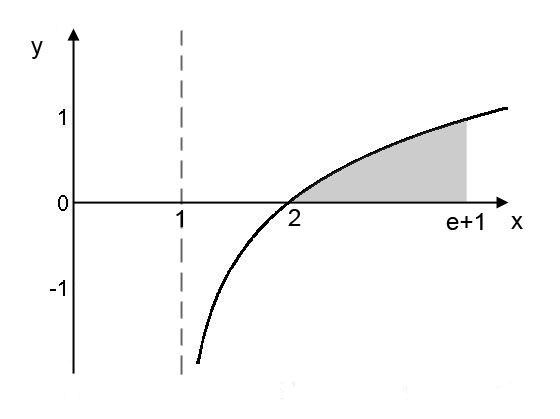
\includegraphics[width=0.55\textwidth]{ImgLog.jpg}
  \end{center}
\end{figure}\\
The region is bounded by the lines $y=0$, $x=1+e$, and by the curve $y=\ln(x-1)$. Using horizontal slices, values of $y$ range from 0 to 1, and values of $x$ range from $e^y-1$ to $1+e$. The double integral becomes
\begin{align*}
  \mathop{\int_{0}^{1} \! \int_{e^y-1}^{1+e}} f(x,y) dydx .
\end{align*}
% ~~~~~~~~~~~~~~~~~~~~~~~~~~~~~~~~~~~~~~~~~~~~~~~~~~~~~~~~~~~~~~~~~~~~~~~~~~~~~~~~~
\item % BOUNDING AN INTEGRAL 
The integrand $f(x,y)$ has the property that 
\begin{align*}
  0 \le \sin(x+y) \le 1,
\end{align*}
because $x+y$ is between 0 and 2, and $\sin(2) < 1$. Then 
\begin{align*}
  0 = \iint\limits_D 0 dA  \le  \iint\limits_D f(x,y) dA \le  \iint\limits_D (1) dA = 1.
\end{align*}
% ~~~~~~~~~~~~~~~~~~~~~~~~~~~~~~~~~~~~~~~~~~~~~~~~~~~~~~~~~~~~~~~~~~~~~~~~~~~~~~~~~
\item % SYMMETRY
\BEN
\item 
Suppose we use the function
\begin{align*}
 h(x,y) & = 11xy.
\end{align*}
Then $h(-x,y) = 11(-x)y = -11xy = -h(x,y)$. 
\item An example of a region that is symmetric about the $y$-axis, but not symmetric about the $x$-axis, is the region bounded by the curves
\begin{align*}
  x = -1,  \quad x = 1, \quad y = 0, \quad y = - 1.
\end{align*}
\item The double integral for our region is
\begin{align*}
  \iint\limits_D g(x,y) dxdy 
  &=  \mathop{\int_{-1}^1 \! \int_{-1}^0} 11xy dydx\\
  &=  -\frac{11}{2} \int_{-1}^1 x dx\\
  &=  -\frac{11}{4} \Big(x^2 \Big)\Big|_{-1}^{1} \\
  &=  -\frac{11}{4} (0)\\
  &= 0.
\end{align*}
\EEN
% ~~~~~~~~~~~~~~~~~~~~~~~~~~~~~~~~~~~~~~~~~~~~~~~~~~~~~~~~~~~~~~~~~~~~~~~~~~~~~~~~~
\EEN % END OF SOLUTIONS
% s~s~s~s~s~s~s~s~s~s~s~s~s~s~s~s~s~s~s~s~s~s~s~s~s~s~s~s~s~s~s~s~s~s~s~s~s~s~s~s~s~s~s~s
% s~s~s~s~s~s~s~s~s~s~s~s~s~s~s~s~s~s~s~s~s~s~s~s~s~s~s~s~s~s~s~s~s~s~s~s~s~s~s~s~s~s~s~s
\subsection{Triple Integrals}

\BEN
% ~~~~~~~~~~~~~~~~~~~~~~~~~~~~~~~~~~~~~~~~~~~~~~~~~~~~~~~~~~~~~~~~~~~~~~~~~~~~~~~~~
\item % TETRAHEDRON
\Emph{Volume of a Tetrahedron} \\
\begin{figure}[h]
  \vspace{-1pt}
  \begin{center}
    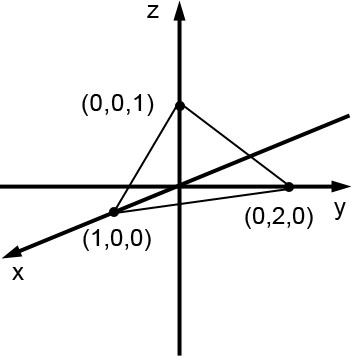
\includegraphics[width=0.35\textwidth]{TetExample.jpg}
  \end{center}
\end{figure}\\
Recall that the volume is the region under the plane $z = 1 - x - y/2$ and over  
\begin{align*}
  R = \{ (x,y) \ | \ 0 \le x \le 1- y/2, \ 0 \le y \le 2 \}.
\end{align*}
Because $z$ lies between 0 and $z = 1 - x - y/2$, the volume, $S$, can be described as
\begin{align*}
  S = \{ (x,y,z) \ | \ 0 \le x \le 1- y/2, \ 0 \le y \le 2, \ 0 \le z \le 1 - x - y/2 \}.
\end{align*}
The volume can be calculated with the triple integral
\begin{align*}
  \mathop{\int_{0}^{2} \! \int_0^{1-y/2} \int_0^{1-x-y/2} }dzdxdy
  &= \mathop{\int_{0}^{2} \! \int_0^{1-y/2}  } ( 1-x-y/2) dxdy\\
  &= \mathop{\int_{0}^{2}  } \Big( x-\frac{x^2}{2}-\frac{xy}{2}\Big)\Big|_0^{1-y/2} dy \\
  &= \mathop{\int_{0}^{2}  } \Big( (1-y/2)-\frac{(1-y/2)^2}{2}-\frac{(y-y^2/2)}{2}\Big) dy \\
  &= \mathop{\int_{0}^{2}  } \Bigg( 1 - \frac{y}{2}-\frac{1}{2}\Big(1 - y + \frac{y^2}{4}\Big)-\frac{y}{2}+\frac{y^2}{4}\Bigg) dy \\
  &= \mathop{\int_{0}^{2}  } \Bigg( 1 - \frac{y}{2} - \frac{1}{2} + \frac{y}{2} - \frac{y^2}{8} -\frac{y}{2}+\frac{y^2}{4}\Bigg) dy \\
  &= \mathop{\int_{0}^{2}  } \Big( \frac{1}{2} - \frac{y}{2} + \frac{y^2}{8} \Big) dy \\
  &= \frac{2}{2} - \frac{4}{4}  + \frac{8}{24} \\
  &= \frac{1}{3}
\end{align*} 
% ~~~~~~~~~~~~~~~~~~~~~~~~~~~~~~~~~~~~~~~~~~~~~~~~~~~~~~~~~~~~~~~~~~~~~~~~~~~~~~~~~
\item % VOLUME OF AN ELLIPSOID
\textbf{Volume of an Ellipsoid}\\
We are given the transformations
\begin{align*}
  x=au, \quad y=bv, \quad z=cw.
\end{align*}
The Jacobian becomes
\begin{align*}   J &=  
  \begin{vmatrix}
   \pxu &  \pxv \\ \\
   \pyu & \pyv \\
  \end{vmatrix}
  =     \begin{vmatrix}
 a&0&0\\
 0&b&0\\
 0&0&c\\
  \end{vmatrix}
  = abc.
 \end{align*}
 The solid enclosed by the ellipsoid is the image of the unit sphere $u^2 + v^2 + w^2 \le 1$. Using that a sphere has volume $\frac{4}{3} \pi r^3$, we find that 
\begin{align*}
  \iiint\limits_{V} dxdydz
  &=  \iiint\limits_{u^2+v^2+w^2 \le 1} abc \ dudvdw \\
  &=  abc \iiint\limits_{u^2+v^2+w^2 \le 1} \ dudvdw \\
  &=  abc (\text{volume of a sphere}) \\
  &=   \frac{4\pi abc}{3} 
\end{align*}

% ~~~~~~~~~~~~~~~~~~~~~~~~~~~~~~~~~~~~~~~~~~~~~~~~~~~~~~~~~~~~~~~~~~~~~~~~~~~~~~~~~
\item % VOLUME OF SOLID
\textbf{Volume of a Solid}\\

\EEN

% s~s~s~s~s~s~s~s~s~s~s~s~s~s~s~s~s~s~s~s~s~s~s~s~s~s~s~s~s~s~s~s~s~s~s~s~s~s~s~s~s~s~s~s
% s~s~s~s~s~s~s~s~s~s~s~s~s~s~s~s~s~s~s~s~s~s~s~s~s~s~s~s~s~s~s~s~s~s~s~s~s~s~s~s~s~s~s~s
\subsection{Change of Variables in Multiple Integrals}

\BEN
% ~~~~~~~~~~~~~~~~~~~~~~~~~~~~~~~~~~~~~~~~~~~~~~~~~~~~~~~~~~~~~~~~~~~~~~~~~~~~~~~~~
\item % GENERAL LINEAR TRANSFORMATION
\Emph{Linear Transformations} \\
\BEN
\item Substituting $v = v_0$ into the linear transformation yields the two equations
\begin{align*}
  x &= c_1u + c_2v_0 \\ 
  y &= d_1u + d_2v_0
\end{align*}
To find the equation of the line in the $xy$-plane, we need to eliminate $u$. There are many ways to do this, but let's multiply the first equation by $d_1$ and the second by $c_1$.
\begin{align*}
  d_1x &= c_1d_1u + c_2d_1v_0 \\ 
  c_1y &= c_1d_1u + d_2c_1v_0
\end{align*}
Subtracting these equations yields
\begin{align*}
  d_1x -  c_1y &=  (c_2d_1 -  d_2c_1)v_0 
\end{align*}
A simple rearrangement gives us
\begin{align*}
  c_1y &= d_1x - (c_2d_1 -  d_2c_1)v_0 .
\end{align*}
Provided that $c_1$ is not zero, we could write this in the form
\begin{align*}
  y &= \frac{d_1}{c_1}x - \frac{c_2d_1 -  d_2c_1}{c_1}v_0 .
\end{align*}
% ~  ~  ~  ~  ~  ~  ~  ~  ~  ~  ~  ~  ~  ~  ~  ~  ~  ~  ~  ~  ~  ~  ~  ~  ~  ~  ~  ~
\item Substituting $x=x_0$ into $x =c_1u + c_2v$ gives us 
\begin{align*}
  x_0 &= c_1u + c_2v,
\end{align*}
Provided that $c_2$ is not zero, 
This is the is mapped into the $uv$-plane REWORD
\EEN

% ~~~~~~~~~~~~~~~~~~~~~~~~~~~~~~~~~~~~~~~~~~~~~~~~~~~~~~~~~~~~~~~~~~~~~~~~~~~~~~~~~
\item % STRAIGHTFORWARD CHANGE OF VARIABLES
The integral can be written as
\begin{align*}
  \iint\limits_R \big(x^2 - y^2\big) dxdy =  \iint\limits_R (x - y)(x+y) dxdy.
\end{align*}
Recall that $R$ is the region bounded by
\begin{align*}
  x+y = 0, \quad x+y = 1, \quad x-y=0, \quad x-y=1.
\end{align*}
The appearance of the terms $(x+y)$ and $(x - y)$ in the integrand and in the lines that bound $R$ suggests the transformation 
\begin{align}
  u & = x+y  \label{zcvzcxvvad}\\
  v &= x - y \label{ntrsraaewvbernst}.
\end{align}
In order to compute the Jacobian, we need explicit expressions for $u$ and $v$. If we add  equations \ref{zcvzcxvvad} and \ref{ntrsraaewvbernst} we find that 
\begin{align*}   x = \frac{u+v}{2}   \end{align*}
And if we subtract equations \ref{zcvzcxvvad} and \ref{ntrsraaewvbernst} we find that
\begin{align*}   y = \frac{u-v}{2}   \end{align*}
The Jacobian becomes
\begin{align*}   J &=  
  \begin{vmatrix}
   \pxu &  \pxv \\ \\
   \pyu & \pyv \\
  \end{vmatrix}
  =     \begin{vmatrix}
 \frac{1}{2} &  \frac{1}{2} \\ \\
   \frac{1}{2} & -\frac{1}{2} \\
  \end{vmatrix}
  = - \frac{1}{4}- \frac{1}{4} = - \frac{1}{2}.
 \end{align*}
We also need to find the limits of  integration in the transformed integral. Using equations \ref{zcvzcxvvad} and \ref{ntrsraaewvbernst} the four lines bounding $R$ in the $xy$-plane become 
\begin{align*}
  u = 0, \quad u = 1, \quad v=0, \quad v=1.
\end{align*}
The double integral therefore becomes
\begin{align*}
  \iint\limits_R \big(x^2 - y^2\big) dxdy 
  &=  \iint\limits_R (x - y)(x+y) dxdy \\
  &=    \mathop{\int_0^1 \! \int_0^1} uv \Bigg|-\frac{1}{2} \Bigg| dudv \\
  &=     \frac{1}{2}\mathop{\int_0^1 \! \int_0^1} (uv) dudv \\
  &=     \frac{1}{2}\int_0^1 \frac{v}{2} dv \\
  &=   \frac{1}{8}.
\end{align*}
% ~~~~~~~~~~~~~~~~~~~~~~~~~~~~~~~~~~~~~~~~~~~~~~~~~~~~~~~~~~~~~~~~~~~~~~~~~~~~~~~~~
\item % CHANGE OF VARIABLES TWICE WITH POLAR
The Jacobian is
\begin{align*}   J &=  
  \begin{vmatrix}
   \pxu &  \pxv \\ \\
   \pyu & \pyv \\
  \end{vmatrix}
  =     \begin{vmatrix}
   3 & 0 \\ \\
   0 & 2 \\
  \end{vmatrix}
  = 6 .
 \end{align*}
We also need to find the limits of integration in the transformed integral. The region $R$ is bounded by the ellipse, $4x^2 + 9y^2 = 36$, which becomes the region bounded by the circle $u^2 + v^2 = 1$. Therefore
\begin{align*}
  \iint\limits_R x^2 \ dxdy &= \iint\limits_{u^2 + v^2 \le 1} (9u^2) 6dudv =  54 \iint\limits_{u^2 + v^2 \le 1} (u^2) dudv
\end{align*}
Switching to polar coordinates, 
\begin{align*}
  u = r\cos\theta, \quad v = r\sin\theta, \quad J = r
\end{align*}
our double integral becomes
\begin{align*}
  54 \iint\limits_{u^2 + v^2 \le 1} (u^2) dudv 
  & = 54 \mathop{\int_0^{2\pi} \!\! \int_0^1} r^3\cos^2\theta drd\theta  \\
  & = 54 \Bigg( \int_0^{2\pi} \cos^2\theta d\theta \Bigg)\Bigg( \int_0^1 r^3 dr \Bigg) \\
  & = 54 \Bigg( \int_0^{2\pi} \frac{1}{2} \big(1+\cos(2\theta) \big) d\theta \Bigg) \Bigg( \frac{1}{4} \Bigg) \\
  & =\frac{27}{4} \Bigg( \int_0^{2\pi}  \big(1+\cos(2\theta) \big) d\theta \Bigg) \\
  & =\frac{27}{4} \big(\theta+\frac{1}{2}\sin(2\theta) \big|_0^{2\pi}  \\
  & =\frac{27}{4} \big(2\pi\big)  \\
  & =\frac{27\pi}{2} 
\end{align*}
% ~~~~~~~~~~~~~~~~~~~~~~~~~~~~~~~~~~~~~~~~~~~~~~~~~~~~~~~~~~~~~~~~~~~~~~~~~~~~~~~~~
\item % SIMPLE CYLINDRICAL WITH CONE
In cylindrical coordinates, the region is described by 
\begin{align*}
  V = \{(r,\theta,z) \ | \ 0 \le r \le 1, 0 \le \theta \le 2\pi, 0 \le z \le 3r \}.
\end{align*}
Our integral becomes 
\begin{align*}
  \iiint\limits_V (r\sin\theta)^2 rdzdrd\theta 
  &=    \mathop{\int_0^{2\pi} \!\! \int_0^1  \!\! \int_0^{3r}} r^3\sin^2\theta dzdrd\theta  \\
  &=   3 \mathop{\int_0^{2\pi} \!\! \int_0^1} r^4\sin^2\theta drd\theta  \\
  &=   \frac{3}{5} \int_0^{2\pi} \sin^2\theta d\theta  \\
  &=   \frac{3}{10} \int_0^{2\pi} \big(1 - \cos(2\theta)\big) d\theta  \\
  &=   \frac{3}{10} \big(\theta - \frac{1}{2}\sin(2\theta)\big) \Big|_0^{2\pi} \\
  &=   \frac{3\pi}{5}
\end{align*}
% ~~~~~~~~~~~~~~~~~~~~~~~~~~~~~~~~~~~~~~~~~~~~~~~~~~~~~~~~~~~~~~~~~~~~~~~~~~~~~~~~~
\item % TRIPLE INTEGRAL IN CYLINDRICAL COORDINATES
In cylindrical coordinates,  $V$ is the region bounded by
\begin{align*}
  0 \le\ &r \le 2 \\
  0 \le\ &\theta \le \frac{\pi}{2}\\
  0 \le\ &z \le \sqrt{4 - r^2}
\end{align*}
The triple integral becomes
\begin{align*}
  \iiint\limits_V dxdydz
  &=    \mathop{\int_0^{\pi/2} \!\! \int_0^2  \!\! \int_0^{\sqrt{4 - r^2}}} r dzdrd\theta  \\
  &=    \mathop{\int_0^{\pi/2} \!\! \int_0^2 } r\sqrt{4 - r^2}drd\theta  \\
  &=   \frac{-1}{3} \int_0^{\pi/2} (4 - r^2)^{3/2} \Big|_0^2 d\theta  \\
  &=   \frac{-1}{3} \int_0^{\pi/2} (0 - 8) d\theta  \\
  &=   \frac{4\pi}{3}
\end{align*}
% ~~~~~~~~~~~~~~~~~~~~~~~~~~~~~~~~~~~~~~~~~~~~~~~~~~~~~~~~~~~~~~~~~~~~~~~~~~~~~~~~~
\item % TRIPLE INTEGRAL IN SPHERICAL COORDINATES
\Emph{Triple Integral In Spherical Coordinates} \\
The solid is a section of a sphere with radius 1, centered at the origin. The section is the part of the sphere that lies above the plane $z=0$, and between the planes $y=0$, and $y=x$. 
\begin{align*}
  \mathop{\int_0^{\pi/4} \!\! \int_{0}^{\pi/2} \!\! \int_0^1 } ( \rho^2 \sin\phi ) \ d\rho\  d\phi\  d\theta
  &=   \mathop{\int_0^{\pi/4} \!\! \int_{0}^{\pi/2} }  \frac{ \sin\phi}{3}  d\phi\  d\theta\\
  &=   \int_0^{\pi/4} \frac{-(0-1)}{3}   d\theta \\
  &=  \pi/12
\end{align*}
% ~~~~~~~~~~~~~~~~~~~~~~~~~~~~~~~~~~~~~~~~~~~~~~~~~~~~~~~~~~~~~~~~~~~~~~~~~~~~~~~~~
\item % EVEN AND ODD
The integral can be written as
\begin{align*}
  \mathop{\int_0^{\pi} \!\! \int_{-1}^1} e^{x^2 + y^2}\sin(y) dydx 
  &= \mathop{\int_0^{\pi} \!\! \int_{-1}^1} e^{x^2}e^{y^2}\sin(y) dydx  = \Bigg( \int_0^{\pi} e^{x^2} dx \Bigg)\Bigg( \int_{-1}^1 e^{y^2}\sin(y)dy \Bigg)  
\end{align*}
The second integral is the integral of an odd function over a symmetrical interval, and so is equal to zero. Therefore,
\begin{align*}
  \mathop{\int_0^{\pi} \!\! \int_{-1}^1} e^{x^2 + y^2}\sin(y) dydx =0.
\end{align*}

% ~~~~~~~~~~~~~~~~~~~~~~~~~~~~~~~~~~~~~~~~~~~~~~~~~~~~~~~~~~~~~~~~~~~~~~~~~~~~~~~~~
\EEN % END OF SOLUTIONS

\end{document}

